\documentclass[12pt]{article}
\usepackage{lmodern}
\usepackage[T1]{fontenc}
%\usepackage[dvips,letterpaper,margin=0.75in,bottom=0.75in]{geometry}
\usepackage[dvips,letterpaper,margin=1in,bottom=1in]{geometry}
\usepackage{cancel}
\usepackage{graphicx}
\usepackage{braket}
\usepackage{latexsym,amssymb,amsmath}
\usepackage{pdfpages}
\usepackage{xcolor}
\usepackage{capt-of}
\usepackage{amsmath}
\usepackage{cite}
\usepackage{lineno}
\usepackage[hyperfootnotes=false,hidelinks]{hyperref}
\usepackage[shortlabels]{enumitem}
\usepackage{pdfpages}
\newcommand{\tcr}{\textcolor{red}}
\newcommand{\tcb}{\textcolor{blue}}

\usepackage[american,fulldiode]{circuitikz}
\tikzset{component/.style={draw,thick,circle,fill=white,minimum size =0.75cm,inner sep=0pt}}

\begin{document}
\ctikzset{bipoles/thickness=1}
\ctikzset{bipoles/length=.6cm}


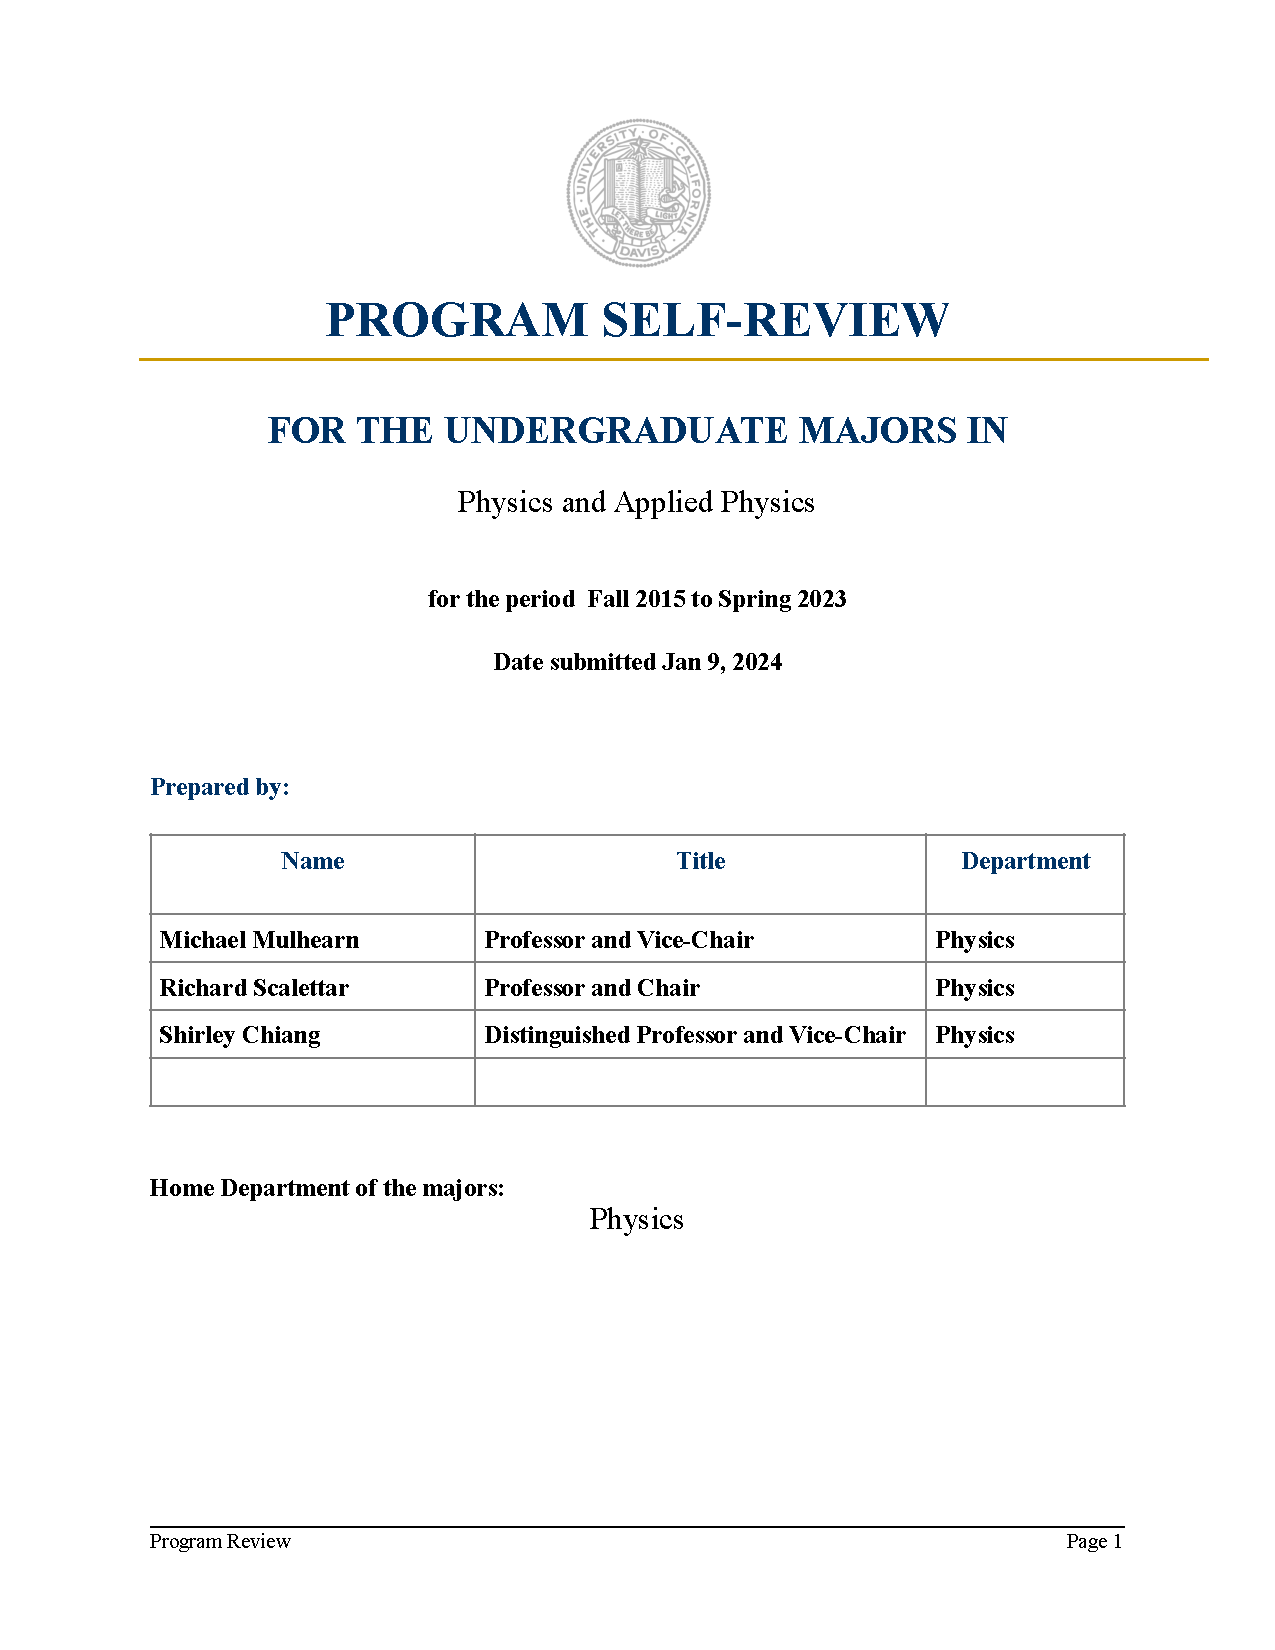
\includepdf[pages=-]{physics_cover.pdf}


% DRAFT ONLY:
%\linenumbers
\tableofcontents

\newpage
\section{Overview of the Majors}
\label{sec:overview}

{\bf Questions: What are the Program Learning Outcomes identified for
  this major? What is the role of this major in undergraduate
  education on the campus, i.e., how does the major contribute to the
  undergraduate educational mission of the campus? Is the major
  clearly distinguished from other similar majors on campus?}\\[3pt]

\noindent
The Department of Physics and Astronomy, and our majors, play a vital
role in the undergraduate education mission of the campus.  Ours is an
ancient discipline, and much of the undergraduate program is spent
learning theoretical and experimental physics from a hundred years ago
or more.  Yet these ideas and concepts remain highly potent in the
modern world, and equally challenging and rewarding to master.  While
studying fundamental physics concepts, our students are exposed to the
latest cutting-edge research and concepts concerning the physics of
the small (nuclear processes, atomic structure, particle searches, and
cellular processes) and the large (dark matter, dark energy,
cosmology).  Our majors are trained in the techniques of experimental
physics, and we have recently dramatically expanded our training in
computational physics.

We are in the process of updating our undergraduate curriculum, as
described below.  The catalog description of the major provides an
accurate overview of the program, and the proposed undergraduate
curriculum update includes changes to the catalog to maintain its
accuracy under the new program.

Our department is distinguished from other departments in the cluster
by the requirement of the most vigorous introductory physics courses,
a diverse upper-level curriculum that develops physics concepts which
appear nowhere else on campus, and a vigorous and sustained emphasis
on fundamental concepts and analytic thinking.  The program learning
objectives specific to our major are described in detail below.\\[3pt]

\noindent
{\bf Undergraduate Curriculum Update (UCU):}
The physics department, led by the undergraduate curriculum committee,
has been developing over the past five years an update to the
undergraduate physics curriculum.  The proposal was subjected to an
extensive vetting process that involved assigned department readers
who were not involved in formulating the initial plan.  The proposal
was unanimously supported by the department in a December 2021 vote.
All new and modified courses have been approved in the UC Davis
Integrated Curriculum Management System (ICMS).  We are working toward
final approval, by campus, of the proposal during AY 2023-2024.

The proposed changes to our program reflect three main observations
about our current program:
\begin{itemize}
 \item Workload over four years of study was imbalanced, with too few
   physics courses in the sophomore year, and too many in the junior
   year.
 \item Integration between transfer students and four-year students,
   who have somewhat different backgrounds, needed to be improved. Our
   recent departmental Climate Survey confirmed this by showing a huge
   satisfaction gap between the groups.
 \item The curriculum did not reflect the explosive growth in
   computational methods and their applications.
\end{itemize}

There are many other aims of the update, but these are the primary
motivations. {\bf The proposed undergraduate curriculum update will be widely
  referenced throughout this document by the acronym UCU.}  The
proposal itself is far too ponderous of a document to include as an
appendix here.  It will be provided as a stand-alone file.  The latest
version of the proposal is also available for download
online\footnote{ See
  \href{https://github.com/mulhearn/classwork/blob/main/curriculum/curriculum.pdf}
  {https://github.com/mulhearn/classwork/blob/main/curriculum/curriculum.pdf
    (click for link)} and use the download option from the pull down menu to view
  the entire document.  }.\\[3pt]
  
\noindent
{\bf Program Learning Objectives (PLOs)}: Although we did not use the
specific term PLO\footnote{We prefer to use the word objectives over
  outcomes, as outcomes could be accidental, whereas objectives are
  intentional.  Fortunately, they both have have the same acronym.} in
that document, these objectives were carefully considered as part of
the development of the UCU (see Sections 4-6 in particular).

There are a number of objectives that are both widely applicable and
central to the discipline of physics, most of which are reinforced in
nearly every physics course that our majors take:
\begin{itemize}
 \item Using logic and analytic reasoning to make predictions.  
 \item Applying general principles (e.g. conservation of energy,
   symmetry) in specific situations.
 \item Testing results using dimensional analysis and limiting cases. 
 \item Dividing complex problems into manageable steps.
 \item Establishing feedback to determine if something is working or not.
\end{itemize}  
The next set of objectives is related to mathematical preparation:
\begin{itemize}
\item Understand the theory and practical application of differential,
  integral, and vector calculus, linear algebra, ordinary and partial
  differential equations.  (MAT 21ABCD, 22AB, and PHY 104A.)
\end{itemize}
While these concepts are first introduced in those courses, they are
continuously reinforced throughout the major.  The next set of
objectives is related to theoretical physics, students are expected
to acquire a working knowledge of the theory and practical application
of the following core topics:
\begin{itemize}
 \item Classical Mechanics (9A/9HA,105AB): the fundamental principles
   of physical laws (e.g. least action and symmetries) are taught in a
   familiar and intuitive context.
 \item Electromagnetism (9C/9HD,110AB): a remarkable special case of
   classical phenomena that anticipate non-Newtonian physics
   (e.g. special relativity, gauge theories).  No other force in
   nature can be understood so completely in such a straightforward
   fashion.  
 \item Quantum Mechanics (9HC/9D,115AB): the rules governing the
   microscopic world are different from those governing our familiar
   macroscopic world.  The rules are not intuitive but they can be
   codified and used to make quantitative predictions which can be
   experimentally verified.
 \item Statistical Mechanics (9HB/9B,9D,112): the crucial statistical
   explanation for how microscopic laws ultimately produce the
   macroscopic world which we inhabit.
\end{itemize}
A major focus of the curriculum update has been to devote more course
work to computational physics.
\begin{itemize} 
 \item Develop programming skills sufficient for tackling problems
   from computational physics (PHY 40,45)
 \item Apply the techniques of computational physics to problems from
   theoretical physics (PHY 110L, 112L, 115L).
\end{itemize}
Our current programming tool set includes Python (first encountered in
PHY 40) and C/C++ (first encountered in PHY 45) but these tools
may evolve over time.  The next set of objectives is related to
experimental physics:
\begin{itemize}
 \item Learn how to conduct and report scientific experiments (PHY 80,
   117, 118, 122A/B, 157).
 \item Gain practical hands-on knowledge of lab equipment,
   electronics, and technical trouble- shooting (PHY 80, 117, 118,
   122A/B, 157).
\end{itemize}
The final objective is for students to apply what they have learned
previously to advanced specialized topics such as nuclear physics,
particle physics, condensed matter, and astronomy.  We refer to these
as capstone courses:
\begin{itemize}
 \item Demonstrate mastery of physics by applying it to advanced
   topics (PHY 129A, 130AB, 140AB, 151-158).
\end{itemize}

\newpage
\section{Outcome of Previous Program Review}
\label{sec:previous}

{\bf Please list the recommendations made at the conclusion of the
  previous review (these may have been made by the review committee,
  Executive Committee and/or Dean) and comment briefly on the current
  status of the matters noted in the recommendations. Discuss any
  other significant changes in the major since the last review.}\\

\noindent
The committee report of the Undergraduate Instruction Program Review
(UIPR) and the Review Team Report from the previous review are
included in the appendix.  These reports were a source of motivation
for the UCU described above, particularly in the specific cases noted
below.  The reports identified strengths in our program, which we
appreciate, but in this overview, we will address only the identified
weaknesses:
\begin{itemize}
 \item {\bf Space, Lab Conditions and Maintenance:} the review team
   was concerned that the undergraduate lab space was ``shabby and in
   need of renovation''.  Within the UC, the cost of building
   renovations is shockingly expensive\footnote{Even by the standards
     of cost-of-living-numbed California residents}, and the
   university funding available for renovations is limited.
   Fortunately, we have received vigorous support from campus with
   several sizable grants for both equipment and renovations, for
   which we are deeply appreciative.  This issue is discussed in more
   detail below (Section~\ref{sec:instruction}).
  
 \item {\bf Transfer Student Readiness:} the review team was concerned
   that many incoming transfer students were not prepared for a
   physics major, and were dropping out or changing major at a high
   rate.  Following the recommendations of the review team and
   committee, we began selective major review in time for academic
   year (AY) 2021-2022.  The department has since seen a substantial
   drop in transfer enrollment at a level that we find potentially
   troubling, if it persists.  This is discussed in more detail below
   (Section~\ref{sec:students}: Students in the major).  {\bf
     Improving the experience for incoming transfer students was a
     major focus of the UCU.}  By ensuring transfer students are
   retained, we hope to mitigate the loss of initial enrollment.

 \item {\bf Computational Instruction:} The review team noted that
   programming course work students were taking outside of the
   department was not adequately training our students in
   computational physics.  {\bf Expanding the role of computational
     physics in our major was a central focus of the UCU} and we have
   added to our curriculum several new required courses focused on
   computation physics.  This is described in more detail below
   (Section~\ref{sec:snws}: Major Strengths and Weaknesses).
  
 \item {\bf Academic Advising:} The review team noted low satisfaction
   with campus and department advising.  In this report, we note that
   student satisfaction with advising has improved.  The likely
   contributions to this improvement, as well as some lingering
   concerns, are described below (Section~\ref{sec:perceptions}:
   Student Perceptions of the Majors).  The size of our undergraduate
   program has increased by $50\%$, but we still have only one
   undergraduate advisor.

 \item {\bf PHY 122: Advanced Physics Laboratory} the review team was
   concerned that students were generally poorly prepared for this
   upper division lab course.  Following the recommendations of the
   committee, we have introduced a new course (PHY 80: Experimental
   Techniques) as a prerequisite for PHY 122.  {\bf As part of the
     UCU, PHY 80 is now a required course for all physics majors (not
     just those taking PHY 122).}  This is discussed in more detail
   below (Section~\ref{sec:snws}: Major Strengths and Weaknesses)
  
 \item {\bf PHY 157:} The review team noted that demand for PHY 157 is
   greater than its capacity.  Regrettably, and despite diligent
   effort by Prof. Tucker Jones in particular, we have struggled to
   maintain the same level of throughput in this course, due to the
   retirement of the previous instructor.  The practical challenges
   here and future plans are discussed below (Section~\ref{sec:snws}:
   Major Strengths and Weaknesses)

 \item {\bf Communication Skills:} The review team reported anecdotal
   evidence of student dissatisfaction with the level of development
   of skills in writing and oral presentation.  PHY 157 and PHY 122
   A\&B currently satisfy one course in the general education
   lower-level writing requirement.  We have recently applied for these 
   courses to satisfy the upper-level writing requirement as currently
   taught, but this has yet to be approved.  If approved, the students
   will be given a choice of satisfying either the lower-division or 
   upper-division requirement.  We discuss this
   issue, along with related concerns about creativity and qualitative
   reasoning, in more detail below (Section~\ref{sec:perceptions}:
   Student Perceptions about the Majors.)
\end{itemize}
We have taken the concerns raised during the previous review quite
seriously, and have made as much progress as we could manage, to the
clear benefit of our department, especially our students.  We
therefore look forward to a fruitful collaboration during this review
as well.

\newpage
\section{Faculty in the Majors}
\label{sec:faculty}

{\bf Questions: Who does the bulk of teaching in the major? What are
  the demographics of instructors in the major? Will the program be
  affected by substantial changes in the faculty (e.g. anticipated
  retirements) in the next review period?}\\[3pt]

\noindent
{\it This and the following sections refer to tables and figures which are available in the
  Appendix.  We use a compact notation, where, for example, [B3]
  refers to Table 3 in Appendix B.}\\[3pt]  

\noindent
Our teaching responsibilities are evenly shared by the faculty, and
the demographics of our course instructors largely reflects the
demographics of our faculty.  A long period of limited hiring has put
the department in an uncomfortable position: new hiring is not keeping
up with retirements and the size of the faculty is shrinking.  This
contraction is occurring when the number of physics majors, and demand
for introductory physics courses by non-majors, are both
increasing.\\[3pt]

\noindent {\bf Rank and Age of Faculty:} There are clear trends
revealed in [B1-2].  The Physics department faculty is significantly
older than the the average for the College of Letters and Science
(L\&S), and the size of the faculty is shrinking.  These trends are
correlated: retirements are out-pacing new hires.  While these numbers
do not reflect our most recent hires (Profs. Matthew Citron and Nancy
Aggawal) this has not been fast enough to avoid a shrinking
department.  Retirements have also left us with no LSOE (i.e. Teaching
Professors with ladder-rank) faculty at present.

A significant obstacle to hiring at an even faster rate is the
availability of startup funding.  Under the current budget model, the
physics department will struggle to maintain a pace of one hire per
year, a pace which would lead to size of the physics faculty shrinking
further.\\[3pt]

\noindent
{\bf Diversity, Inclusion, and Equity:} The data provided in [B3-5] is
incomplete, so we will address the topic of diversity of the faculty
in purely qualitative terms.  Most importantly, our faculty is
overwhelming supportive of taking strong measures to improve the
diversity of our faculty within the limits of what we are legally
allowed to do.  We are not looking for quick and easy fixes.  Instead,
we have been studying and adopting best-practices in hiring.  For
example, our two most recent faculty searches were intentionally
broadened in scope, as this has been shown to increase the diversity
of the applicant pool.  As another example, we have started providing
zoom interview questions in advance, as well as more details about the
interview process in general, because evidence shows that members of
URGs are systematically disadvantaged when such details are assumed to
be already known.  As is often the case when adopting best practices,
we found that these steps have also made the interview process better
overall. For example, when provided with the questions in advance,
applicants gave better, more thoughtful, and more useful responses.
This remains an urgent issue, and there remains much to be done
here.\\[3pt]

\noindent
{\bf Discussion Checklist:} 
{\it The program was provided with an
  explicit list of items to discuss.  To increase readability, we
  discuss the salient issues in the most natural order first.  At the
  end of end of each section, we include a ``Discussion Checklist'' which
  indicates where each discussion point was covered, using the
  original enumeration (For example, "a-e") of topics provided in the original
  prompt. We have omitted the original prompt to increase
  readability.}\\[3pt]
  (a-e) Discussed above [B1-5].\\[3pt]

\newpage
\section{Instruction, Advising, and Resources in the Majors}
\label{sec:instruction}

{\bf Questions: How effective is the delivery of instruction in the
  major? Are faculty engaged in the major? Is advising adequate? Is
  there adequate staff support? Are adequate space and facilities
  available? Is the program keeping pace with developments in the
  field? Are grading standards appropriate? What is the role of
  virtual and hybrid courses in this major? Please attach or include
  here a sample 4 year graduation plan for your program.}\\[3pt]

\noindent
Our highly-engaged faculty is dedicated to delivering effective instruction to our students, and we adhere to rigorous academic standards with respect to grading.  However, the size of our faculty is shrinking while the number of physics majors is increasing, which is putting a serious strain on our ability to deliver instruction.  The size of our staff, including undergraduate advising, has remained constant during the review period, and is struggling to keep up with increasing demands on their time.  Our space and facilities are adequate for our purposes, but could be improved.  These issues are discussed in more detail below.

Undergraduate physics is largely focused on the
cutting-edge theoretical physics of a hundred years ago or more.  Yet
we do stay relevant in the modern world: those old ideas remain
challenging to master and highly potent to cutting-edge applications.
Our multi-year continuing commitment to the UCU is strong evidence
that we continue to innovate.  One exception: outside of emergencies,
we have no plans to include virtual or hybrid courses in our program,
as we have found, for our discipline, that no reasonable amount of
effort can produce such a course which is as effective as learning in
person (See Section~\ref{sec:remote}).  Sample four-year graduation
plans (as well as two year plans for transfer students) are provided
for every major and specialization, in the UCU.  See Table 6 in that
document, for one example.\\[3pt]

\noindent
{\bf Grading Policy:} The grade distribution in [B12]
\footnote{This is our compact notation for Table 12 in Appendix B}
shows that physics (and chemistry) are grading significantly more strictly than
L\&S overall, which is a conscious decision on our part.  Our
adherence to rigorous academic standards adds significant value to the
physics degree, and to physics course work in general.  For example,
our top students are regularly accepted into top graduate programs,
likely in part because the A's they receive in our courses represent a
meaningful accomplishment.  We are concerned about the ability of UCD
to continue as a forefront research institution and engine of social
mobility if the grade inflation that we see in L\&S overall is allowed
to continue or accelerate.  Our students are at a disadvantage for
receiving graduation honors because the thresholds are set
unattainably high due to grade inflation elsewhere.  In L\&S seniors 
are permitted to do an Honors thesis if their GPA falls
in the top 16\% (Currently 3.846).  Less than 8\% of our seniors
typically fall above this overall GPA, or less than half the overall
number.\\[3pt]

\noindent
{\bf Instructors:} Our department prioritizes providing physics majors
with ladder faculty instructors, particularly for upper-division
course work.  The student FTE per faculty FTE is increasing [B6].
This is the result of both an increase in the number of physics majors
and a decrease in the number of faculty.  Despite the challenges from
a shrinking faculty, physics majors are being taught by ladder faculty
[B9-10] for $90\%$ of their upper division course work, a larger
fraction than any other L\&S department considered this cycle.  They
are being taught by ladder faculty for $58.5\%$ of their
lower-division physics course work, also above average for L\&S.

For introductory physics course work, we also utilize the
highly-effective pedagogy of Continuing Lecturers.  Dr. Dina
Zhabinskaya manages the PHY 7 series (introductory physics aimed at
bioscience) and Dr. Thomas Weideman manages the PHY 9 series (introductory
physics aimed at natural science and engineering).  They are both
deeply committed to innovative pedagogy, are great assets to our
department, and regularly share their wisdom with the rest of the
faculty.  We regularly hire Unit-18 pre-Six Instructors (temporary
lecturers) as well.  Some of our graduate students are interested in
more extensive teaching experience than typical TA assignments afford,
and, when we believe they are up to the challenge, we also hire
Associate Instructors to teach in PHY 7 and 9.\\[3pt]

\noindent
{\bf Staff Support:} Physics is a unique discipline with its own
unique culture, and we are profoundly grateful to the staff members
that work alongside us to maintain it.  During the review period, we hired Chris Brainerd as a replacement for the head of the instructional support unit.  Brainerd is a former PhD candidate at UCD and he brings expertise in electronics, physics analysis, and a knack for troubleshooting table-top experiments.  He is providing excellent support to the advanced undergraduate labs. The overall size of our staff has remained constant during the review period, while the number of majors has increased.  Thousands of non-majors take our introductory physics courses each year, and these students access the staff as well.  For example, students often reach out to staff for advice when they have trouble scheduling their first-choice lecture section.  Given the huge number of students involved, this can be quite significant even for seemingly straightforward requests.  As the number of non-physics majors at UCD is also increasing, our staff is facing growing demand for services from both majors and non-majors alike.   Our staff is increasingly reliant on triage: keeping up with only the highest priority issues while leaving other important issues unsettled.\\[3pt]

\noindent
{\bf Instructional Space, Equipment, and Facilities:} While total
assignable space has increased [B11], it has not been faster than the
number of student FTEs has increased.  The overall amount of assignable
space is above average for L\&S, but this reflects our need for
dedicated laboratory space, and large lecture halls adjacent to
demonstration support.  As discussed in Section~\ref{sec:previous},
the previous review noted a deficiency in the condition of the lab
space used for undergraduate instruction.  Fortunately, we have
received vigorous support for new instructional equipment and renovation of instructional space.  The campus allocated over \$300,000 toward refreshing the PHY 7 discussion lab classrooms in the Earth and Planetary Sciences building.  The department received an award\footnote{These awards are in the form of 80\% match to the departments 20\% contribution.} of \$307,000 to expand the physics teaching labs from Roessler into the Physics Building and to update instructional equipment.  This award is also supporting the relocation and update of the computer lab from room 106 Physics to room 289 Physics.  We expect the renovations and lab moves to be completed in summer 2024.  The department received an award of \$21,000 to replace the CCD camera for astronomy labs.  We have an additional request for \$15,000 to replace telescopes for the lower division astronomy labs that is still pending.\\[3pt]

\noindent
{\bf Collaboration with other programs: } Physics (like Mathematics)
is a foundational discipline for most Science, Technology,
Engineering, and Math (STEM) disciplines.  Nearly every STEM
discipline trains its students in our introductory physics courses.
Physics itself is a rather unique discipline, and we have little
competition from other fields to consider.  Instead, we focus on
collaboration, which is much more useful.  We have a wide range of
applied physics majors which afford students the opportunities to
study complementary specialized topics (e.g. computer science,
atmospheric science) outside of the department.  The UCU strengthens
those majors by affording more flexibility with a more expansive list
of specialized courses to choose from.  Our new course work in
computational physics (particularly PHY 40: Introduction to
Computational Physics, a course with no college-level prerequisites)
focuses on the bare minimum of programming techniques necessary to
tackle challenging physics problems (See Section~\ref{sec:snws}).  It
moves quickly from ``introductory programming'' to ``computational
physics''.  This makes the course highly complementary to course work
in the Computer Science and Engineering department, and the markedly
different emphasis may be of interest to other disciplines as
well.\\[3pt]

\noindent
{\bf Discussion Checklist:} (a) Discussed above [B6].  (b) According
to table [B7] only about $70\%$ of students enrolled in upper division
physics courses are physics majors.  We suspect this is inaccurate,
most likely double majors are not being handled correctly.  But we
would certainly be delighted if 30\% of our upper-division students
were from other majors! (c) There is an expected increase [B8] in the
number of TAs that resulted from new courses, particularly PHY 80, PHY
40 and PHY 45, which require significant TA support for lab sections,
as well as the addition of discussion sections to some core upper
division courses.  (d-e) Discussed above [B9-10]. (f) Discussed above
(Instructional Space, Equipment, and Facilities) (g) Discussed above
[B12] (h) Discussed above (introductory remarks) (i) Discussed above
(Staff Support) (j) Staff advising is discussed in
Section~\ref{sec:perceptions} (Academic Advising).  (k) Discussed
above (Instructional Space, Equipment, and Facilities) (l) Discussed
above (introductory remarks) (m) Discussed above (Collaboration with
other programs) (n) Discussed above (introductory remarks).

\newpage
\section{Students in the Majors}
\label{sec:students}

{\bf Questions: This section is intended to characterize the students
  in this major. How have enrollments in the major varied over the
  period of the review, in terms of both the numbers and quality of
  the students? Are students succeeding in the major both in terms of
  qualitative and quantitative academic standards? Are students
  graduating on time? Are there impacted classes (e.g., with limited
  offerings or long wait-lists) or other bottlenecks that
  unnecessarily impede student success? How do students find out about
  the major?  Is the major reaching a wide and diverse spectrum of
  students? Are students who enter the major retained in the major,
  and if not, why not?}\\[3pt]

\noindent
As described in detail below, during this review period, the
undergraduate program has grown in both size and diversity.  We
believe there is strong demand by students for excellent physics
programs, and by employers for those we train.  With sufficient
resources, our department could grow further to meet that demand.  We
hope that we continue to grow in Diversity as well.  By most of the
measures of student academic achievement which we consider below,
physics students are performing just slightly below the average for
L\&S, which is a notable accomplishment given that physics courses are
graded significantly more stringently than L\&S on average.  The most
concerning metrics are a dramatic drop in transfer student admissions
to eight total in AY 2022-2023, and a four-year time-to-graduation for
$73\%$ of physics majors, which is significantly lower than for L\&S
overall (85\%).  The UCU includes a number of changes to our program,
including the removal of bottlenecks, that we expect to impact these
and other metrics.  However, it is too soon to judge their efficacy.
Looking at the available metrics all together, we see that our program
is successful at attracting, retaining, and graduating students.

The primary source of information about our major is the department
website, the UC Davis course catalog, and the undergraduate academic
advisor.  We do considerable outreach with our students to keep them
on track.  This is all discussed in more detail in
Section~\ref{sec:perceptions} under ``Academic advising''.\\[3pt]

\noindent
{\bf Size of the undergraduate program:} The number of physics and
applied majors has been growing, as the result of a mutual agreement
between the university and department to begin admitting about $50\%$
more students into the program starting in AY 2019-2020.  This amount
was targeted as the maximum number of additional students that physics
could handle without the need for additional lecture sections in core
physics courses.  This increase is the main trend evident in 
[B13]\footnote{This is our compact notation for Table 13 in Appendix B}
and [B17]. Taking applied physics and physics together, the number of
international students in physics [B25] has increased by roughly
$25\%$, consistent with the increase in L\&S.  To accommodate the
increase in the number of students, we added TA-led discussion
sections to some of the upper-division physics course courses, which
is something physics majors had been requesting even before the class
size increase.  These tables also put the ratio of applied physics to
physics majors historically at 1:2, but of late the share of applied
physics majors appears to be growing.\\[3pt]

\noindent
{\bf Diversity of physics majors:} Combining physics and applied
physics majors, the fraction [B15] who are women has increased just
slightly during the review period, while the fraction of women in L\&S
overall has decreased by about $3\%$.  Again combining physics and
applied physics majors, the fraction [B16] who are from
underrepresented groups (URGs) has increased from $14\%$ to $19\%$.
When the number of majors is accounted for, the increase in the number
of women is not statistically significant, but the increase in the
number of students from URGs is statistically significant.\\[3pt]

\noindent
{\bf Double majors and minors:} There has been a noticeable increase
in the number of physics majors who are double majors [B14] but the
rate is still lower than the average for L\&S.  This lower rate is the
combination of unit caps on the amount of total course work a student
can take (imposed by L\&S) coupled to the hierarchical structure of
most science disciplines.  In our experience, double majors in physics
have little flexibility left in their schedule to pursue other
interests and electives, so we generally do not advise them.  We do
heartily encourage minors, but yet few physics majors complete one
[B24].\\[3pt]

\noindent
{\bf Transfer students and their experience:} As discussed in
Section~\ref{sec:previous}, the previous review was concerned that a
large number of incoming transfer students were not prepared for a
physics major.  Following the advice of the review committee, the
department started selective review of transfer students in time for
AY 2021-2022.  Our hope is that by selecting students who are more
likely to succeed as physics majors, we will continue to graduate
transfer students as physics majors at approximately the same rate,
while dramatically reducing the number of students who drop out of the
program.  A major focus of the UCU was improving the experience of
transfer students, by leveling out their course work in the first year
to avoid a ``brick wall'' of intense course work that previous
students faced in their first quarter.  It is too early the judge the
effectiveness of any of these changes.

Omitting AY 2020-2021 from consideration due to the pandemic, we see
that since AY 2021-2022 there has been a significant drop [B18] in the
number of new transfer students, the result of a drop in applications
and the tighter admission requirements of selective major review.
Prior to selective major review, we would generally have
120-130 applicants in a typical year.  Of those accepted, 30-35 students would
start as physics majors, but only 10-12 would remain as
physics majors past the first year.  In recent years, applications
have fallen to as low as 90 students, and about 75\% of
students pass selective major review.  In AY 2022-2023, we had about
eight new transfer students [B18] but in AY 2023-2024 (not in the
appendix data set), we had 13 new transfer students.  If we retain
these students through graduation, we should not observe any reduction in
the number of transfers that graduate as physics majors, despite the
reduction in our acceptance rate.

A significant number of transfer students in applied physics and
physics require an additional year to graduate: only $22\%$ of applied
physics majors and $41\%$ of physics majors graduate in two years as
intended [B22].  This is significantly lower than $64\%$ for L\&S
overall.  Improving this experience for transfer students was a major
focus of the UCU.

It is too soon to draw any conclusions about the changes to our
program that we have made which impact transfer students.  However, we
have made a request for reports of additional metrics pertaining to
transfer students.  We plan to scrutinize these statistics to judge
the impact and efficacy of these changes to our program.  We are also
considering outreach to community colleges to boost the application
rate.  These considerations fall within the scope of our departments
DEI efforts as well, as many students from URGs access the university
through their community colleges.  It is vital that we maintain a
viable path for transfer students through our program.\\[3pt]

\noindent
{\bf Student Academic Performance:} The average GPA [B19] of physics
and applied physics majors is around 3.2 but varies as low as 2.8 and
as high as 3.3 depending on the class and major.  This is slightly
lower than the average for L\&S (3.3).  This likely reflects the fact
that physics majors take more physics courses, which we have already
established are generally graded more stringently than courses from
other departments in L\&S.  In [B20] we see qualitatively similar
results with respect to the fraction of students in good standing,
which ranges from $79\%$ to $94\%$ depending on the class and major,
and is slightly lower than L\&S overall.  We see a slight increase in
degrees conferred [B21], for both physics and applied physics majors.
When the data for AY 2023-2024 are available, we should start to see
an increase due to the larger number of physics majors.

Looking at time to graduation [B23] for students that remain physics
majors the entire time, we see that $83.3\%$ of applied physics majors
and $72.7\%$ of physics majors graduate within four years as planned.
That rate for physics majors is significantly smaller than the average
for L\&S (84.5\%).  This is integrated from 2016 to 2022, which makes
it somewhat difficult to interpret.  We should monitor this metric
over the next few years to see if there is a persistent problem here
to address.  We do expect that time-to-graduation for nominal
four-year students should decrease as a result of the changes in the
UCU, which includes changes that remove stalling out of four-year
students in their sophomore year.  But it is too soon to judge the
efficacy of these changes.\\[3pt]

\noindent
{\bf Discussion Checklist:} (a-m) Discussed above [B13-25] (n-o)
Discussed above (introductory remarks).

\newpage
\section{Student Perceptions of the Majors}
\label{sec:perceptions}

{\bf Question: What are current students' and recent graduates'
  opinions of the major? }\\
  
\noindent
Our students' opinions of the physics and applied physics majors are
for the most part consistent with college averages, within the limited
statistics available from survey responses.  In the discussion that
follows, we note some areas of encouragement and concern, and include
anecdotal data where pertinent.\\[3pt]

\noindent
{\bf Interpretation of student feedback:} Soliciting feedback from
students is a useful and important diagnostic tool, but the results
must be carefully interpreted.  We know that student evaluations
reflect significant implicit biases\footnote{See, for example:
  Kreitzer, Rebecca J. \& Sweet-Cushman, Jennie. Evaluating Student
  Evaluations of Teaching: a Review of Measurement and Equity Bias in
  SETs and Recommendations for Ethical Reform. Journal of Academic
  Ethics 20 (1):73-84 (2021).}  and are strongly correlated with
student perceptions of their course grades.  For example (referring
to [B12] and [C29]\footnote{This is our compact notation for Figure 29 in Appendix C} 
 ) we are not surprised to see that a department which
is an outlier with respect to grading ($85\%$ of letter grades are
A's) is also an outlier with respect to student satisfaction with
faculty instruction ($88\%$).  In the physics department, $33\%$ of
letter grades are A's and student satisfaction (amongst junior and
senior physics majors) with faculty instruction is a more modest
$67\%$.  We should not conclude that the other department is
performing any better (or worse, for that matter) than the physics
department, only that our approaches are different, likely reflecting
the different needs of our students.\\[3pt]

\noindent
{\bf Limited Statistics from Alumni Responses:} We also need to be
careful not to draw sharp conclusions from samples with limited
statistics.  There were few responses collected from physics alumni:
three from applied physics majors and 17 from physics majors.  We have
carefully checked all of the alumni responses [C12-22], [C31-36],
[C41-43], and [C49-54].  Amongst the questions, the only ones which
yielded a statistically significant deviation from the college average
were:
\begin{itemize}
  \item Questions [C18], [C21] and [C22] none of which we found to be
    illuminating.
  \item Questions [C31] and [C32] where we do see (borderline)
    statistically significant dissatisfaction with the grading system
    and use of information technology.
  \item Question [C43] which references peer advisors, which we do not
    have in physics.
\end{itemize}

\begin{table}[htbp]
\caption{\label{tbl:appc} Survey results from Appendix C, using
  results from freshman through seniors, combining results from
  physics and applied physics majors. The sample size is N=61 from
  which a binomial statistical uncertainty has been calculated.
  Results as a percent are organized by question (Q) and the results
  for physics and applied physics majors (Physics) are compared to the
  College (L\&S).}
\begin{center}
\begin{tabular}{|lll|lll|lll|lll|}
\hline
Q & Physics & L\&S & Q & Physics & L\&S & Q & Physics & L\&S & Q & Physics & L\&S \\
\hline
% Binomial Uncertainty:
C1 & 90 $\pm$ 4 & 91 & C5  & 55 $\pm$ 6 & 64 & C23 & 53 $\pm$ 6 & 76 & C38 & 55 $\pm$ 6 & 52 \\
C2 & 91 $\pm$ 4 & 90 & C6  & 71 $\pm$ 6 & 74 & C24 & 84 $\pm$ 5 & 68 & C39 & 56 $\pm$ 6 & 47 \\
C3 & 79 $\pm$ 5 & 85 & C7  & 57 $\pm$ 6 & 60 & C25 & 84 $\pm$ 5 & 73 &     &            &    \\                  
C4 & 89 $\pm$ 4 & 93 & C8  & 78 $\pm$ 5 & 79 & C26 & 82 $\pm$ 5 & 76 & C44 & 46 $\pm$ 6 & 37 \\
~  &            &    & C9  & 30 $\pm$ 6 & 46 & C27 & 48 $\pm$ 6 & 61 & C45 & 52 $\pm$ 6 & 56 \\
~  &            &    & C10 & 68 $\pm$ 6 & 69 & C28 & 39 $\pm$ 6 & 49 & C46 & 41 $\pm$ 6 & 54 \\
~  &            &    & C11 & 69 $\pm$ 6 & 69 & C29 & 52 $\pm$ 6 & 66 & C47 & 55 $\pm$ 6 & 59 \\
~  &            &    &     &            &    & C30 & 75 $\pm$ 5 & 61 &     &            &    \\
\hline 
\end{tabular}
\end{center}
\end{table}

\noindent
{\bf Maximizing Statistical Uncertainty from Student Responses:} To
maximize the sample size from current students, we have included all
years in the survey result (the default results include only juniors
and seniors).  We have also computed a weighted average of the
responses from both applied physics and physics majors.  This combined
sample has a size of N=61 (with a slight variation from question to
question that has been neglected from our analysis) from which we
estimated a naive binomial statistical uncertainty.  The results are
reported in Table~\ref{tbl:appc}.\\[3pt]

\noindent
{\bf Understanding of the major:} Using the combined survey results in
Table~\ref{tbl:appc} we see that understanding of the major [C1],
program requirements [C2], program policy [C3], and accuracy of the
catalog [C4] were all comparable to the L\&S average, with the last
two being low by about one standard deviation.  Even though there is
therefore no statistically significant evidence to support the claim,
we do suspect there may be some student confusion in the context of
the UCU.  For example, we have begun teaching newly approved courses,
even though they are not yet required by the major, as the UCU has not
yet reached final approval.  We have done our best to communicate the
situation to our students, and we are encouraging them to take the new
courses even though they are not required yet.  We would not be
surprised if some confusion exists in this context.  We plan to
complete the approval process and make the necessary catalog updates
as soon as possible, at which point we are confident that any
confusion will begin to dissipate.\\[3pt]

\noindent
{\bf Satisfaction with major:} Using the combined survey results in
Table~\ref{tbl:appc}, we see that the responses from our majors
regarding fair treatment [C6], faculty access [C7], ability to get
into major [C8], library resources [C10], and overall satisfaction
[C11] were all consistent with college averages within statistical
uncertainty of the survey sample.  As discussed above, there are no
statistically significant results from the alumni survey that warrant
further discussion.

Our majors were less satisfied ($30\% \pm 6\%$) than the college
average ($46\%$) with respect to [C9] ``Education enrichment
programs''.  In the current program, it is nearly impossible for our
majors to study abroad, which likely contributes to the observed
student dissatisfaction.  In the UCU, four-year students have
sufficient flexibility that more students may find it feasible to
study abroad.  The department does provide other sources of education
enrichment, such as student research, and it would be illuminating to
probe student satisfaction with specific avenues of enrichment.

Our majors were less satisfied ($55\%\pm6\%$) than the college average
($64\%$) with respect to [C5] the ``faculty being open to discuss
students' needs, concerns, and suggestions''.  Even though this is
just barely more than one standard deviation from the college average,
it is disappointing to learn that so many students feel this way.
This is something we should consider as a faculty.\\[3pt]

\noindent
{\bf Satisfaction with Instruction:} Using the combined survey results
in Table~\ref{tbl:appc} we see that our majors believe plagiarism is
not being adequately explained [C23].  We encounter plagiarism most
frequently in physics courses through the use of online websites, such
as Chegg, to provide answers to homework questions.  There is growing
evidence that using sites such as Chegg for cheating expanded during
the pandemic and hasn't receded.  We wonder if the low score here is
reflecting student and faculty disagreement as to what constitutes
plagiarism, or, conversely, if it indicates students' concerns that we
are not doing enough to discourage and condemn this relatively new
form of cheating.  Clearly more discussion between students and
faculty is needed about cheating.

The results of [C24-26] show that students believe they are well
practiced in recalling, explaining, and analyzing concepts, methods,
and ideas.  However, when it comes to qualitative judgment [C27] and
creativity [C28] physics majors reported lower than average practice,
which we discuss further below.

Our majors are quite well satisfied with their TAs ($75\% \pm 5\%$)
compared to the college average ($61\%$).  This is heartening, if not
surprising.  TA's are most often cast in roles which directly support
students, helping them work through their homework problems in
discussion sessions, for example.

Satisfaction with faculty is lower ($52\% \pm 6\%$) than the college
average ($66\%$).  This is concerning and warrants a closer look at
the data.  If we consider physics majors only, and restrict ourselves
to junior and seniors, we see 67\% are satisfied with faculty
instruction, just a bit higher than the college average.  Further
investigation confirms that the heightened dissatisfaction comes from
two contributions: current freshman and sophomores, and all applied
physics majors.

One major difference between applied physics and physics majors is the
amount of course work that is taken outside of the department. We are
well aware of the frustration that applied physics majors are facing
in completing their course work outside of physics.  Perhaps part of
the dissatisfaction stems from this.  The UCU aims to give applied
physics majors more flexibility which we hope will improve this
situation.  In any event, it is clear that additional outreach with
applied physics majors and physics majors in lower division courses is
needed to determine the root causes of this elevated
dissatisfaction.\\[3pt]

\noindent
{\bf Academic Advising:} The satisfaction of alumni with advising was
all consistent with the college average, within the statistical
uncertainty of the sample.  The only exception was a question
regarding peer advising, which the physics department does not provide.  
Amongst our majors, using the combined
sample of Table~\ref{tbl:appc}, we see that students are satisfied
with the quality of academic advising (55\% $\pm$ 6\%) slightly higher
than the college average (52\%) and with access to academic advising
(56\% $\pm$ 6\% ) higher than the college average (47\%).  Only the
latter is (borderline) statistically significant.

These results are encouraging.  As discussed in
Section~\ref{sec:previous}, low satisfaction with advising was noted
by the previous review.  We believe we understand the source of the
improvement, based on our own anecdotal data from individual student
interactions.  Most importantly, Prof. Boeshaar runs a physics career
seminar and Prof. Knox runs an alumni speaker seminar.  These are not
required courses, but the scope of discussion extends to
academic advising, particularly for subjects that students are
concerned about.  Secondly, the staff undergraduate advisor, Amy Folz
and the vice-chair for the undergraduate program, Prof. Mulhearn, have
devised a highly effective triage system, whereby frequently encountered issues are
handled by Folz, and more complicated problems are immediately kicked
up to Prof. Mulhearn.  We have found this arrangement to be quite
effective.  Folz also arranges multiple annual outreach events (pizza
nights) which provide a forum for academic advising.  Prof. Mulhearn
is an annual speaker in the physics career seminar.  Lastly, a
significant number of students participate in undergraduate research,
and research advisors are a natural source of academic advice as well.
Our attempts to impose a more top-down assigned faculty advisor had
lackluster results, with a clear lack of student and faculty interest,
which was compounded by the pandemic.  Fortunately, it seems that our
more organic, fully optional avenues for academic advising are proving
to be effective.  Prof. Boeshaar is continuing to play her pivotal
role past her recent retirement, but we cannot expect this to continue
indefinitely.\\[3pt]

\noindent
{\bf Course Offerings:} Using the combined data sample from
Table~\ref{tbl:appc}, we note that our students rated access to small
class sizes [C44] higher (46\% $\pm$ 6\%) than the college average
($37\%$).  Our students rated the availability of courses needed to
graduate [C46] at lower (41\% $\pm$ 6\%) than the college average
(54\%), and this lower level of satisfaction is present for both
physics and applied physics majors.  Anecdotally, we are aware that
applied physics majors struggle to schedule outside course work.  We
are addressing this problem in the UCU by increasing the number of
choices available to applied physics majors for their course work
outside of the department.  We are also discussing with the computer
science department the possibility to give higher priority to our
applied physics (computational physics) majors in their impacted
courses.  We are also aware that physics majors struggle to schedule
advanced physics labs, and we are attempting to improve throughput in
these courses as well.  We offered a fall section of advanced physics
lab for the first time in AY 2023-2024.  We have also begun
renovations to provide more space, and are adding additional lab
modules, toward increasing the number of students in each section.
Our students rated the availability of general education courses [C45]
and the variety or courses [C47] at levels consistent with the college
average within the statistical uncertainty of the sample.  The alumni
responses were all consistent with the college average within the
statistical uncertainty of the sample.\\[3pt]

\noindent
{\bf Communication, Creativity, and Qualitative Judgment:} Oral and
written communication was mentioned as a concern in the previous
program review.  Our students gain experience in scientific writing by
writing lab reports in their experimental physics courses.  One area
where we could probably add more practice with writing is in student
homework.  We generally grade homework looking for just enough steps
to show the student understood the problem.  We could easily assign
students longer write-ups for specific problems, in which they would
need to explain what they are doing in a clear and concise manner.  If
done correctly, this might actually make homework easier to grade!

When it comes to oral communication, this immediately runs into
several practical challenges.  With a throughput of order 60 students
per year, even having each student provide a 15 minute presentation
would be a commitment of 15 hours: 50\% of a standard lecture course.
That's a big time commitment, and one we cannot afford in our core
required course work.  However, many instructors of upper division
specialty courses include oral presentations as part of their
curriculum.  We also note that students are free to choose about 50\%
of their undergraduate course work, so they could take ``CMN 001:
Introduction to Public Speaking'' as just one of many possible avenues
for gaining additional practice in oral communication.

We saw above that when it comes to qualitative judgment [C27] and
creativity [C28] physics majors reported lower than average practice.
This is disappointing, if not entirely surprising.  A large fraction
of the undergraduate physics degree is invested toward understanding
well-established theories which were mostly developed a century ago or
more.  Problems for these theories which have exact analytic solutions
are limited, and so students invest a lot of time solving problems
that have already been solved for a century or more as well.  This
paints perhaps too bleak a picture, as instructors do labor to breathe
life into their subjects every quarter, but they are facing strong
headwinds, and these results most likely reflect those headwinds.  One
area of the undergraduate physics degree where creativity and
qualitative judgment are more naturally exercised is in computational
physics and experimental physics.  Here students devise and debug
their own code or experimental apparatus, and face new problems not
constrained to those with exact analytic solutions.  It will be
interesting to see if the improvements and increased focus on these
subjects in the curriculum update will lead to students getting more
practice in these topics.\\[3pt]

\noindent
{\bf Discussion Checklist:} (a-e) Discussed above [C1-52].

\newpage
\section{Post-Graduate Preparation}
{\bf Questions: How well does the major prepare students for
  postgraduate education and careers?  Do the students have
  opportunities to meet and work with faculty outside the classroom
  setting? Is there sufficient support for internships or experiential
  learning opportunities?  Are there ample opportunities for students
  to learn about career options?}

\begin{table}[htbp]
\caption{\label{tbl:appcii} Survey results from Appendix C, using
  results from only junior and seniors, combining results from physics
  and applied physics majors. The sample size is N=37 from which a
  binomial statistical uncertainty has been calculated.  Results as a
  percent are organized by question (Q) and the results for physics
  and applied physics majors (Physics) are compared to the College
  (L\&S).}
\begin{center}
\begin{tabular}{|lll|}
\hline
Q & Physics & L\&S \\
\hline
% Binomial Uncertainty:
C54 & 60 $\pm$ 8 & 46 \\ 
C60 & 90 $\pm$ 5 & 74 \\
C75 & 49 $\pm$ 8 & 42 \\ 
C76 & 58 $\pm$ 8 & 65 \\ 
C77 & 62 $\pm$ 8 & 62 \\ 
\hline 
\end{tabular}
\end{center}
\end{table}

\noindent
Our students' rate their opportunities for undergraduate research
[C54]\footnote{This is our compact notation for Figure 54 in Appendix C}
 and their plans for further academic study [C60] significantly 
higher than the college average.  The difference is
large enough as to be statistically significant even considering the
limiting sample size of the survey.  They rated faculty access (in
various ways) [C75-77] as comparable to college averages, within the
statistical uncertainty of the survey sample.\\[3pt]

\noindent
{\bf Limited Statistics of Survey Data:} The limited statistics in the
survey data from physics alumni renders [C55-59],[C61-74],[C78-80] of
limited use and they are not considered here.  Following the procedure
of the previous section, we have computed the weighted average of
responses from applied physics and physics majors in
Table~\ref{tbl:appcii}.  Because these questions pertain to issues
that tend to arise later in each student's career (such as undergraduate
research) we have included only juniors and seniors, which limits the
sample size to $N=37$.\\[3pt]

\noindent
{\bf Preparation for the Workforce:} Absent statistically significant
results from the alumni surveys, we can consider our own anecdotal
data.  Many faculty maintain contact with their former students long
after they graduate.  This keeps us well informed about issues related
to workforce preparation.  The networks of former students that
faculty develop are an extremely valuable tool for helping newly
graduated students enter the workforce\footnote{In some cases, we have
  former students interviewing former students!}.  A recurring theme
is that the advanced labs (PHY 122, 117, 118, and 157) were amongst most
valuable learning experience the student encountered.  We are
optimistic that our investment in computational physics will yield
similar feedback in the future.\\[3pt]

\noindent
{\bf Discussion Checklist:} (a) Discussed above [C54], (b) Discussed
above [C60], (c) Discussed above (Preparation for Workforce), (d)
Discussed above [C75-77].

\newpage
\section{Educational Objectives and Assessment}

{\bf Question: How does the program monitor and evaluate its success
  in achieving its Program Learning Outcomes (Section 1)?}\\[3pt]

\noindent
The PLOs for our majors are defined in Section~\ref{sec:overview}
along with specific courses which reinforce those objectives.  We have
not historically hosted these objectives publicly, but as this has
been requested as part of the review we are planning to do
so. 

Responsibility for monitoring the effectiveness of our program at
enabling our students to reach these objectives lies with the
vice-chair for the undergraduate program and the undergraduate
curriculum, in collaboration with the physics faculty.  As part of the
curriculum update, we have developed a new procedure for continuously
monitoring, discussing, and revising the curriculum.  Each spring, the
undergraduate curriculum committee organizes a faculty meeting devoted
entirely to the undergraduate program.  The instructors of core
undergraduate courses prepare short summaries of their courses,
covering how they taught the course, including notable differences
from example syllabi which we now maintain, and any observed
shortcomings in student preparation from prerequisite courses.  If any
changes to the example syllabi are needed, the UGCC prepares new
versions, and the faculty votes on whether or not to adopt the new
versions.

The acquisition of PLOs related to mathematics and theoretical physics
are most directly assessed through in-person final exams in core
courses (e.g. 104A, 105AB, 110AB, 112, 115AB).  The faculty members
that teach core courses are generally able to immediately spot
short-comings in student progress from the final exam performance.
The experimental physics PLOs are assessed mainly through student lab
reports.  Instructors of PHY 80 have also recently introduced a lab
practical examination which we have found to be quite successful.

Professors engaged in teaching our new computational physics courses
are learning new pedagogy appropriate to that discipline.  We have
become quite found of Parsons problems, which have students provide
the correct ordering of (scrambled) lines of code, in order to meet a
given prompt.  Not only are these a fast and practical means for
evaluating programming abilities in person, they also train students
to ``compile in their head'' instead of relying (as many new students
do) on trial and error.  We also evaluate submitted programs, but we
are concerned, in the long run, that students might get by on simply
copying existing solutions, unless we have an effective means of
in-person evaluation.

This self-review is synergistic with the years of prior effort that
our department has invested in understanding the performance of our
program, and proposing improvements.  The strengths and weaknesses we
have identified are summarized in Section~\ref{sec:snws} and our
future plans in Section~\ref{sec:future}.  However, we heartily
encourage the reviewers to read through the UCU proposal document.  It
is rather long, but it represents years of effort on our part.\\[3pt]

\noindent
{\bf Discussion Checklist:} (a-g) Discussed above.

\newpage
\section{Major Strengths and Weaknesses}
\label{sec:snws}

{\bf Summarize the major overall strengths of the program as well as
  any current problems that you perceive.}\\[3pt]

\noindent
All happy departments are alike; each unhappy department is unhappy in
its own way.  Fortunately, ours is a happy department, and so our
strengths are those fairly universal ones.  We have a collegial
faculty that works well together, allowing each faculty member to
effectively add their unique talents and interests.  Our staff are
dedicated and effective.  Our students are diligent and inquisitive,
and they support one another.  They are remarkably empathetic.
Together we have built an impressive and productive departmental
culture.

Our small class sizes and an active undergraduate research program
promote strong ties between faculty and students.  Our students
receive a considerable amount of personal attention both in and out of
class.  We have an exceptionally varied offering of advanced
undergraduate specialty courses, the work of a dedicated faculty
directed at its students.\\[3pt]

\noindent
{\bf Physics Club:} We have an active student-led physics club that organizes social activities for physics majors, provides tutoring in introductory physics, and performs an annual Physics show during UC Davis Picnic Day that generally mixes demos with an engaging script.\\[3pt]

\noindent
{\bf TEAM-UP}:
The department joined the TEAM-UP project in 2020.  The goal of TEAM-UP is to at least double the number of bachelor’s degrees in physics and astronomy awarded to African American students by 2030.
TEAM-UP has sponsored a Transfer Student Peer Mentoring Program at UC Davis which help transfer students with the transition from their community college to UC Davis.  In AY 2023-2024 there were 12 mentors and 14 mentees in the program.\\[3pt]

\noindent
{\bf Computational Physics:} Our curriculum now includes a substantial
number of required computational physics courses.  In PHY 40
(Introduction to Computational Physics) students learn the basics of
Python and then move directly into solving numerical and physical
problems using computational methods.  In PHY 45 (Computational
Physics) they are introduced to C++, without much concern for advanced
language features, and tackle more advanced physics problems based on
their course work in introductory physics.  Later, they take 2-3
one-unit computational lab courses, designed to work alongside their
upper division course work.  Much of the earlier computational physics
problems focused on mechanics; now they use computational physics to
tackle problems from upper division quantum mechanics, electricity and
magnetism, and statistical mechanics. These courses are just the core.
As the faculty gains confidence in our students' computational
abilities, we should see computational physics spread throughout our
program.  We cannot make every physics major a computer scientist any
more than we can make every one a mathematician, but we can make every
physics major as effective at solving physics problems with computer
programs as they are with calculus.\\[3pt]

\noindent
{\bf Experimental Physics:} Following the advice of the previous
committee, we have introduced PHY 80: Experimental Techniques to
better prepare students for the PHY 122A: Advanced Lab in Condensed
Matter Physics and PHY 122B: Advanced Lab in Particle Physics.  We
developed a course that introduces basic laboratory equipment, analog
electronics (up to the diode), introductory statistics, experimental
uncertainty, and analysis and presentation of experimental data.
After learning these techniques, primarily through lab activities,
students apply them to the measurement of fundamental constants like
the speed of light and Planck's constant.

As part of the UCU, we have made PHY 80 a required course for every
physics major (not just those taking 122A/B).  We have adjusted the
other upper division lab courses to take advantage of it: the 116ABC
sequence (Electronic Instrumentation) has been replaced with PHY 80,
PHY 117 (Physics Instrumentation with Analog and Digital Electronics)
and PHY 118 (Physics Instrumentation for Data Acquisition).  The latter
two courses can be taken in any order, and are in a nearly continuous
state of renewal by Prof. Prebys, in order to take advantage of new
technology (such as systems that host programmable digital logic and a
CPU on a single chip) well suited for students.

Unlike the setups for the lab exercises in PHY 80, 117, and 118,
which are easily duplicated, each experiment in PHY 122A, 122B, and
157 generally uses a unique custom designed apparatus.  The
complicated nature of these experiments also requires a lot of personal
attention from the professor teaching the course.  For all of these
reasons, the throughput in these advanced lab courses is limited, and
requires precise rationing by the undergraduate advisor to ensure
students can finish the course in time to graduate.  We are making
several changes in an attempt to increase throughput.  We taught our
first fall section of 122A in 2023, which was feasible as a result of
scheduling and prerequisites changes which are part of the UCU.  If we
add a third 122B section, these changes alone will increase throughput
by 50\%.  However, finding professors that are qualified and willing
to teach these extremely demanding courses is a challenge.  We have
also begun renovations of the first floor of physics, to provide space
for additional experimental setups, which should allow us to increase
the number of students in each section.  However, we must take care
not to reduce the amount of personal attention students receive in
this lab, or make it even more demanding for the instructors.

The throughput in PHY 157 is even more limited, due to other practical
considerations such as the time of year during which weather is
favorable for observation, safety concerns which limit the number of
people that can be on the roof for observation, and limited faculty
qualified to teach the course.  With the retirement of Prof. Tony
Tyson, Prof. Tucker Jones has been teaching the course, but we have
struggled to maintain throughput, let alone increase it.  The department recently received a donation of new observatory equipment, valued at \$175,000, which includes three new telescopes: an Astro-Physics RH 305, an Astro-Physics 155mm Starfire EDF, and a computer-controlled f/11 14-inch Celestron.  These new telescopes will relieve one major bottleneck to the throughput in PHY 157.\\[3pt]

\noindent
{\bf Unit Caps:} A course with three hours of lecture per week
at UC Davis usually rates as three units\footnote{Most of our physics courses
  are actually rated as four unit courses, due to extensive problem
  solving in the homework.}.  Four-year students typically graduate
with around 180 units, and students must receive special permission to
register for any more classes once they reach 225 units.  {\bf Within
  L\&S, we are allowed to require a maximum of 110 units in our
  majors.} Prerequisite courses, even those outside our department,
count toward this maximum.  This unit cap places severe limitations on
what we can do with our program.

The ostensible reason for the unit cap is to allow sufficient time for
students to explore areas of interest outside of their major.  We are
sensitive to that consideration, but find that this mixture is too
lean (on major course work) for our purposes.  Our students invest a
great deal of time in prerequisite course work, and by the time they
are ready to take on advanced course work in physics we run into the
unit cap.

The situation is even more dire for applied physics majors.  We must
make substantial cuts in core physics material (such as second quarter
in mechanics and quantum mechanics) simply to make space for required
course work outside of their major.  Offering a degree that combines
two scientific disciplines is extremely difficult, effectively
impossible for bio-physics, and while we do have a chemical physics major,
it is quite limited in the amount of required upper-division chemistry.
Achieving a double major in two scientific disciplines is also nearly
impossible due to the limit of 225 units on total course work.

A degree in physics dducation would help address a major societal
need, particularly in California where currently many high school
physics teachers are retiring.  However, the large number of education courses and teaching experiences
required make it impossible to complete significant upper-division course work in physics while remaining below the cap.

We propose a compromise: lower-division prerequisite course work {\bf
  outside the host department} should count at a pro-rated amount of
50\% toward the 110 unit cap.  This would ensure that our students
have plenty of exposure to course work outside of physics, while
giving us some breathing room for advanced course work.  It would
enable us to develop applied physics majors that are much more useful
to our students.  By limiting the concession to additional
lower-division course work, it should help preserve a feasible
two-year path to graduation for transfer students.

\newpage
\section{Future Plans}
\label{sec:future}
{\bf Describe current or proposed plans to strengthen educational
  objectives of the program, such as increasing enrollments, improving
  student performance, and increasing the contribution of the program
  to the campus educational objectives. Comment on the long term
  strategy or goals regarding hybrid and virtual instruction in this
  program. Describe and justify if new resources are needed to
  preserve or strengthen the program.}

Our most immediate future plans for the undergraduate program are
centered on receiving final approval and finishing the implementation
of the UCU.  Following that, we will want to monitor the performance
of the program carefully.  Of particular importance are the impact of
selective major review and the curriculum changes on transfer
students.  Ideally we will see that we continue to graduate at least
10-12 transfer students in physics each year, with hardly any leaving
the program.

We have an annual faculty meeting devoted to a review of the
undergraduate program, and evaluating the impact of the UCU will be a
central topic for the next few years at least.  We will likely want to
make small further adjustments.  This process has given us expertise
in the various tools for updating course descriptions and catalog
copy, and so we would like to invest some time in bringing those up to
date as well.  The scope of the undergraduate curriculum update did
not include introductory physics (PHY 7 and PHY 9) so we plan to
tackle those next.

We see our substantial investment in computational physics as merely a
start.  Our hope is that professors will take further advantage of
student expertise in computational physics as it becomes more
reliable.  For when you solve a problem by calculating an analytic solution and writing
a computer program, and your solutions agree, then you have gained both
understanding and confidence.

The biggest challenge facing our department is the decrease in the
size of the faculty, because hiring is not keeping up with
retirements.  While the faculty is shrinking the demands on our
department are increasing.  We have more physics majors, but also more
undergraduate students taking our introductory physics courses.  We
need substantial investments from campus to dramatically increase our
hiring rate.  Here the main hold-up is startup.  And yet these
retirements are saving campus enormous sums of money.  If we direct
some fraction of those savings toward start-up expenses of new hires,
we could likely avert disaster for our department.  One or more LSOE
(Teaching Professor) hires would also help address our instructor
shortage without the need for large startup funding.  We also need more
investment in staff.  We have only one undergraduate student advisor
on the faculty who is severely taxed to keep up with not only our
majors, but the myriad of issues that arise with the {\em thousands}
of students that take introductory physics each year.

\newpage	
\section{Minors}
{\bf Please comment on the minors currently administered by your
  department.}\\[3pt]

\noindent
The department offers a minor in physics which 1-3 students complete
each year.  The objective for the physics minor is to provide an
opportunity for students to gain a meaningful understanding of physics
concepts and expertise in putting them to practical use, but without
committing to an entire degree.

The requirements for the minor are quite simple to state: students
must complete six upper division physics courses (excluding a small
set of ineligible courses, e.g. independent study).  However,
achieving this minor is quite challenging due to the hierarchical
nature of our course work.  Upper division course work generally
requires completing six courses in mathematics, four courses in
introductory physics, and many courses further require PHY 104A (Math
Methods in Physics).  This large number of prerequisites likely
discourages many students.  And those that have completed these
prerequisites for their own major are likely already science majors,
and therefore see little benefit to a physics minor.

We believe the physics minor is well designed for those relatively few
students dedicated enough to their interest in physics to pursue it.  We see no need
to make adjustments and we accept that demand for the minor is small.

\newpage
\section{Emergency Remote Instruction}
\label{sec:remote}

{\bf The review team, UIPRC, and UGC understand that the emergency
  remote instructional environment required by the COVID-19 pandemic
  presented extraordinary demands on department faculty, staff, and
  students. Please address the successes and challenges faced by your
  program during emergency remote instruction. Provide information
  about any new practices that were beneficial and the program plans
  to continue, as well as any practices and outcomes that fell short
  of your standards.}\\[3pt]

\noindent
Our faculty made a heroic effort during the COVID-19 pandemic, but the
quality of instruction suffered tremendously nonetheless.  In
qualitative terms, we saw that the top 1/3 of students managed
reasonably well with remote instruction, but the bottom fell out for
the remaining 2/3.  We believe we saw a dramatic increase in cheating,
and there is growing evidence that it has not receded.  We also
believe that we are still seeing residual effects of the pandemic on
current students.  Specifically, the level of mathematical preparation
and study habits have not fully recovered to pre-pandemic levels.
These are subjective evaluations, but they have been widely observed
by our faculty.

During emergency remote instruction, student engagement dropped
precipitously.  Early advice to instructors urged us to provide
asynchronous course work as much as possible, to accommodate students
that might struggle, under the circumstances, to connect at a fixed
time.  We soon discovered, however, that fully asynchronous courses
were a disaster for student engagement and morale.  Most of our instructors
quickly reverted back to fully live (via zoom) lectures, or a mixture of
{\bf short} asynchronous pre-recorded lectures\footnote{Video hosting
  sites which monitor viewer engagement over time showed that students
  generally drop out of pre-recorded lectures after about ten minutes}
punctuated with live in-person discussions.

For faculty teaching lab courses, the burden was even greater.  These
are crucial experiences for our students, and faculty generally went
to extraordinary lengths to provide kits or other means for students
to gain some hands on experience.  This generally required redesigning
entire courses with little notice.

During live (via zoom) lectures, instructors were generally faced with
a wall of blankness: students nearly universally leave their cameras
off, and deeply resent being forced to turn them on.  With few
exceptions, faculty despised remote instruction.  But we did our best.

And despite all of these efforts, there was no meaningful equivalency
between the online courses we provided and our traditional in-person
courses.  Any instructor has seen that students that do not attend
lecture generally become demoralized, detached, and perform well below
their abilities.  COVID-19 forced something like that onto every
single one of our students.  May we never have to do that again.

\end{document}
